\documentclass[../Main/Knit.tex]{subfiles}

\section{Pacific Biosciences: Isoform Sequencing}

\subsection{Introduction}
For successful DNA polymerisation, the DNA polymerase requires high concentration of nucleotides to allow high accuracy and processivity.  However for sequencing, this limits sensitivity to detect each labelled base incorporation and respective fluorophore emission, due to high background noise level. In the past, second-generation sequencing technologies have circumvented this issue by the step-wise addition, scan and wash of each set of labelled nucleotides, but at a compromise of read length. 

Unlike RNA-Sequencing, Pacific Bioscience’s Single Molecule Real Time sequencing (SMRT \nomenclature{SMRT}{Single Molecule Real Time sequencing}) is able to generate long reads is due to its ability to mimic natural, uninterrupted, processive DNA synthesis, through three important innovations \cite{Eid2009}: 
\begin{enumerate}
	\item Creation of a circular template, SMRTbell, enclosed with hairpin adapters at end of the inserted target double-stranded DNA, allowing uninterrupted DNA polymerisation \cite{Travers2010} (Figure \ref{fig:smrtbell}).
	\item Sequencing of each SMRTbell with a bound polymerase at the bottom of a nanometre-wide well (zero-mode-waveguide - ZMW \nomenclature{ZMW}{Zero-Mode-Waveguide}), and all wells contained within a single SMRT chip\cite{Levene2003}. Due to the very nanoscale size of the ZMW and reduced detection volume, a single nucleotide incorporation can be sensitively detected against the high background of labelled nucleotides, achieving a high-signal-to-noise ratio (Figure \ref{fig:mechanism})).  
	\item Addition of phospholinked nucleotides, each labelled with a different colour fluorophore corresponding to the four different bases (A, C, G and T), which allows for natural, accurate and processive DNA synthesis\cite{Mccarthy2010} (Figure \ref{fig:Phospholinked_Nucleotides}).
\end{enumerate}
In summary, SMRT sequencing detect fluorescence events that correspond to addition of one specific nucleotide by a polymerase attached to the bottom of a tiny well. 

\begin{figure}[h!]
	\centering
	\vspace{50pt}
	\begin{subfigure}{0.3\linewidth}
		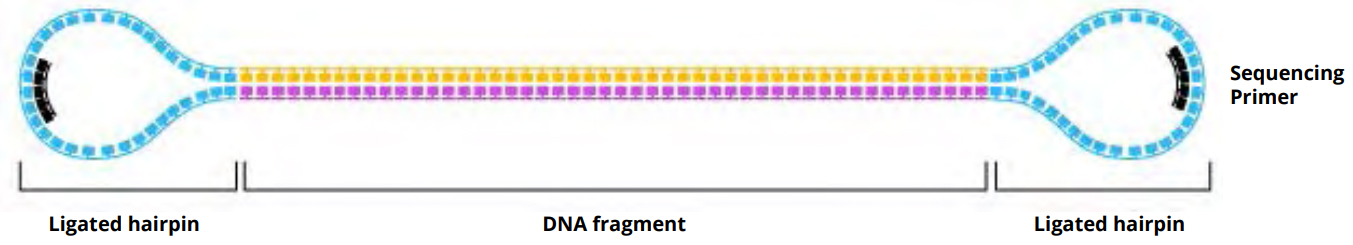
\includegraphics[width=\linewidth, height=0.05\textheight]{Pictures/Smrt_template.jpg}
		\caption{SMRT-bell template}\label{fig:smrtbell}
	\end{subfigure}
	\vspace{20pt}
	\hspace{5em}
	\begin{subfigure}{0.4\linewidth}
		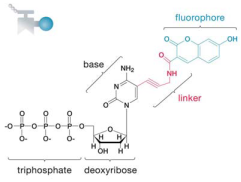
\includegraphics[width=\linewidth, height=0.2\textheight]{Pictures/Phospholinked_nucleotides.png}
		\caption{Phospholinked Nucleotides}\label{fig:Phospholinked_Nucleotides}
	\end{subfigure}
	\vspace{20pt}
	\begin{subfigure}{0.8\linewidth}
		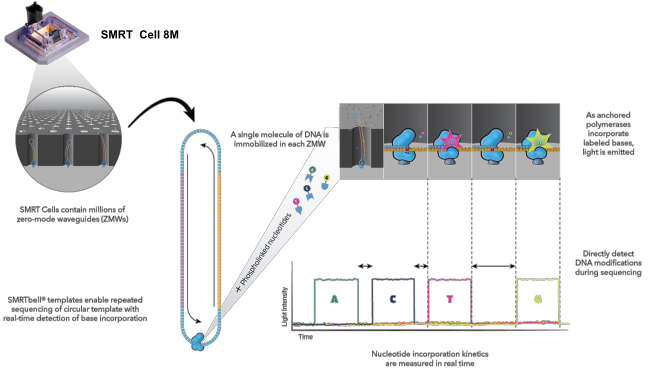
\includegraphics[width=\linewidth, height=0.3\textheight]{Pictures/Mechanism.png}
		\caption{PacBio Single-molecule real time sequencing}\label{fig:mechanism}
	\end{subfigure}
	\captionsetup{width=0.95\textwidth}
	\caption[PacBio SMRT]%
	{\textbf{PacBio SMRT}: At time of writing, PacBio released Sequel II with the provision of an 8M chip, containing 8 million wells, each capable of sequencing one single molecule. Figures adapted from PacBio}
	\label{fig:Mechanism}
\end{figure}

Currently, PacBio offers two sequencers: Sequel I and Sequel II; RSII was the first commercially available sequencer, but is no longer supported. With Sequel v2 chemistry from 2017, fragments longer than 10kbp were typically only read once and had a single pass accuracy of 58-87\%. Last 3 years have seen teh release of 1 instrument (Sequel II), 4 chemistries (Sequel v2,v3, Sequel II v1, v2) and 4 versions of the SMRT-Link analysis suite.  

\subsubsection{Mechanism}
Due to the circular nature of the SMRT bell, the polymerase can continually read through the insert, sequence the same DNA template multiple times and generate a continuous sequence of bases (continuous long read, CLR or polymerase read), which contains the hairpin adapter sequences. Pending on the polymerase lifetime and insert length, both strands can be sequenced multiple times, or “passes” in a CLR, which can then be delineated by the adapter sequences and resolved to multiple reads (subreads). These subreads can be further collapsed to yield a highly-accurate Circular Consensus Sequence (CCS\nomenclature{CCS}{Circular Consensus Sequence}), increasing the accuracy of individual raw subreads from 85\% to 99\% of the consensus read, proportional to the number of passes \cite{Travers2010}.

Reads from PacBio are therefore not a set length, as with short-reads generated by RNA-Seq, but a distribution of lengths dependent on the library size and the polymerase activity \cite{Ardui2018,Rhoads2015}. However with previous chemistries, there was a bias towards sequencing molecules of a certain length due to preferential loading of SMRTbell templates - loading by diffusion favoured shorter molecules\cite{Loomis2013} whereas loading using Magbeads allowed proportional loading to the concentration rather than by length, but prevented sequencing of molecules <1kb. Previous attempts to mitigate this loading problem have been to fractionate the library by length (size selection) and enrich for longer cDNA molecules before sequencing \cite{Au2013}, but this approach is more expensive and laborious. Thankfully, recent improvement in the technology and chemistry (v3.0) with usage of molecular crowding agents have alleviated the short-read bias and resulting the magbead loading method obsolete \cite{Oikonomopoulos2020}.   

%https://www.pacb.com/wp-content/uploads/2015/09/Guide-Pacific-Biosciences-Template-Preparation-and-Sequencing.pdf
\begin{figure}[h]
	\centering
	\vspace{20pt}
	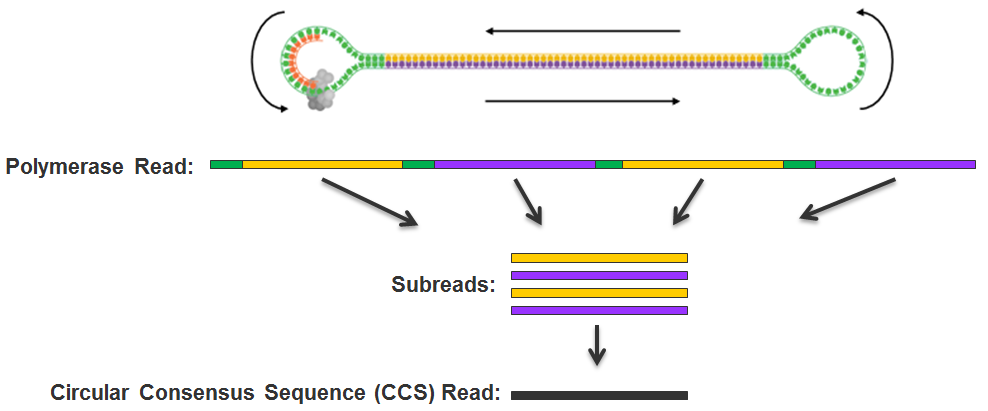
\includegraphics[width=0.8\linewidth, height=0.2\textheight]{Pictures/SMRTAdapter.png}
	\captionsetup{width=0.95\textwidth}
	\caption[Generation of Circular Consensus Sequence]%
	{\textbf{Generation of Circular Consensus Sequence}: CCS is generated by the collapse of multiple subreads, which sequence correspond to the double-stranded cDNA of interest. The greater the number of "passes" sequenced by the polymerase, the longer the polymerase read, the more subreads generated, and subsequently the higher the quality of CCS. Picture adapted from PacBio}
	\label{fig:CCS}
\end{figure}


\subsubsection{Performance and Run Quality Metric}
In an ideal situation, all the wells will contain an insert that will generate a positive signal. However, because XXXX, there will be some wells that are empty (quality metric denoted as P0: Productivity 0), and some wells that will be overloaded with multiple inserts with more than one polymerase (quality metric denoted as P2: Productivity: P2). Thus only wells that contain one polymerase (denoted as P1, Productivity 1) will generate a positive signal. Overloading may lead to increase in output of yield per SMRT cell, but increases the chance of P2 (multi-loaded ZMWs), resulting in shortened read lengths and lower accuracy compared to single-loaded ZMW. Loading can be optimised through titration.  	

A good run is defined by 50-70\% P1, a >XX kB polymerase read-length. Over-loading (>70\%) may result in reduced base quality (noisy base-calling), whereas under-loading (<50\%) results in lower throughput. A short polymerase read-length indicates sequencing/library preparation issues. These metrics are dependent on chemistry, pre-extension, and movie-runtime. 